\chapter{Results}
\label{chap:Results}
\begin{figure}[ht]
    %\centering
    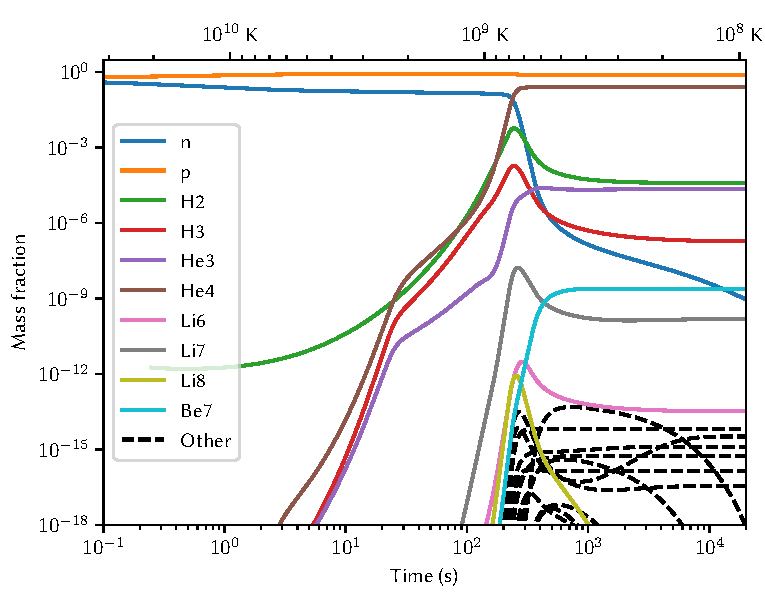
\includegraphics[width=5.1in]{figures/abundancelight.pdf}
    \caption{Time evolution of light nuclei abundance during BNN, with mass fraction technically being the close approximation $X_i=Y_i A_i$. }
    \label{fig:lightXevo}
\end{figure}
Running the code creates a complete overview of abundance evolution as shown on figure \ref{fig:lightXevo}. As expected neutrons protons and deuterium remain in equilibrium for the first few seconds. As the temperature decreases, deuterium abundances slowly increase quickly followed by tritium and both helium isotopes. Here the dominant nuclear reactions are neutron captures creating tritium, and converting ${}^3$He to ${}^4$He, which continues until around 230 seconds. At this point the rate of deuterium creation is finally great enough to have a significant impact on neutron abundance, which until then had remained almost unchanged since the $p\leftrightarrow n$ rates fell out of equilibrium. This leads to a rapid drop in neutron abundance creating a bottleneck on the production of deuterium and tritium, which in turn slows down and eventually stops the production of ${}^3$He and ${}^4$He. Without these light nuclei lithium abundances also drop, as reactions such as ${}^4\text{He}+{}^3\text{H}\rightarrow {}^7\text{Li}$ become outmatched by the proton captures ${}^7\text{Li}+\text{p}\rightarrow 2{}^4\text{He}$ and ${}^6\text{Li}+\text{p}\rightarrow {}^7\text{Be}$. Conversely, Beryllium 7 is primarily destroyed via neutron capture ${}^7\text{Be}+\text{n}\rightarrow {}^7\text{Li}+\text{p}$, and therefore sees a rapid increase in abundance immediately after the drop in neutrons.
\begin{figure}[ht]
    %\centering
    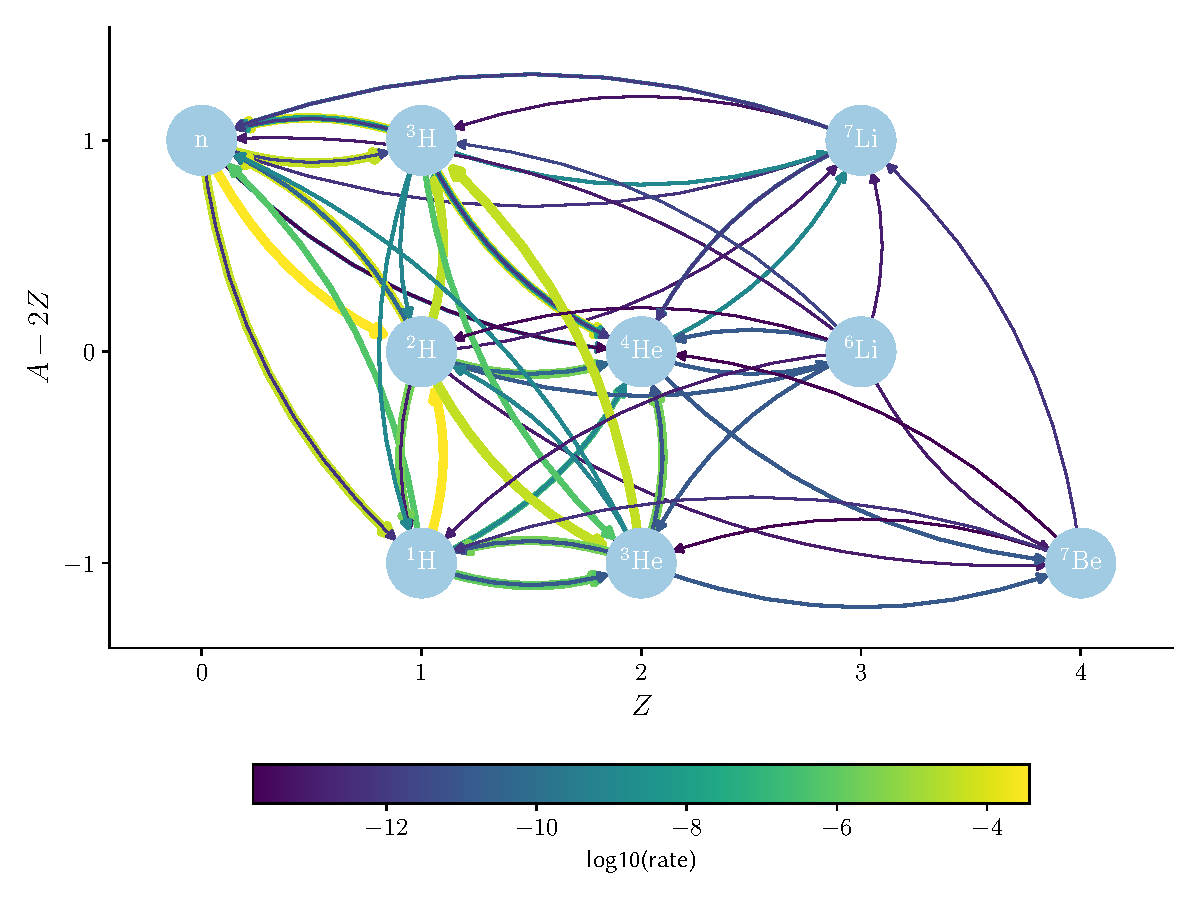
\includegraphics[width=5.1in]{figures/smallnet5minutes.pdf}
    \caption{Reaction rates 5 minutes after Big Bang at \num{7.6e8} K. Only including rates within 10 orders of magnitude of strongest.}
    \label{fig:5minutenet}
\end{figure}

The relations of these reactions are illustrated in figure \ref{fig:5minutenet}. This snapshot is taken immediately after the aforementioned drop in neutron abundance with $Y_n=0.2\%$. Despite this $n+p\rightarrow d$ is still the strongest reaction, followed by reactions creating ${}^3$He and ${}^3$H. 

Equal d and n mass fraction
The 

\begin{figure}[ht]
    %\centering
    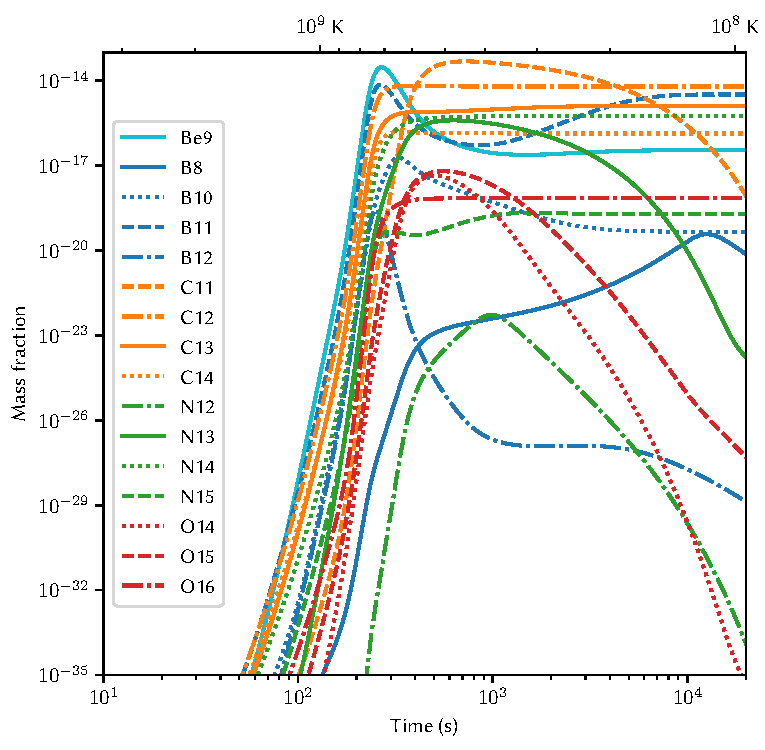
\includegraphics[width=5.1in]{figures/abundanceheavy.pdf}
    \caption{Time evolution of heavy nuclei abundance during BNN, with mass fraction technically being the close approximation $X_i=Y_i A_i$.}
    \label{fig:heavyXevo}
\end{figure}



\subsection{Dominant reactions}





\section{Precision}
Throughout the code there are several numerical 



\subsection{Electron energy}

\subsection{Tolerances}

\subsection{Interpolation}

\subsection{Initial time}

\subsection{}


\section{Comparison with AlterBBN}
\label{sec:Altercompare}



\section{Final abundances}

\section{Nuclear solutions to the Lithium problem?}